\section{Auswertung}
\label{sec:Auswertung}
\subsection{Bestimmung des Geometriewinkels}
\begin{figure}[H]
    \centering
    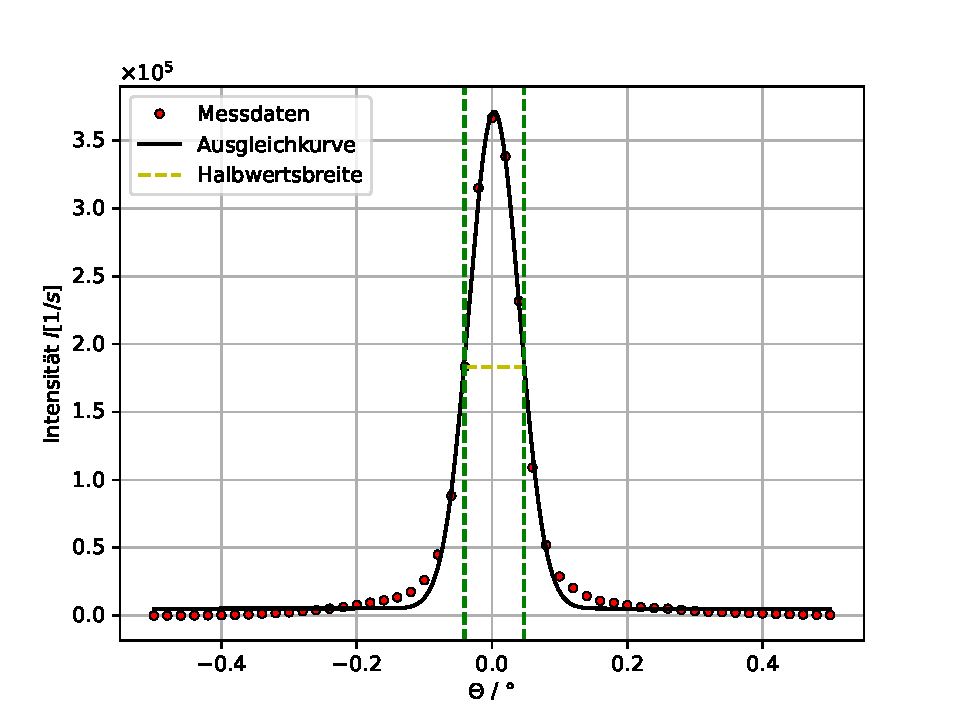
\includegraphics[width=0.8\textwidth]{plots/Detectorscan.pdf}
    \caption{Winkelabhängigkeit der Intensität des Röntgenstrahls}
    \label{fig:Detectorscan}
\end{figure}

\begin{figure}[H]
    \centering
    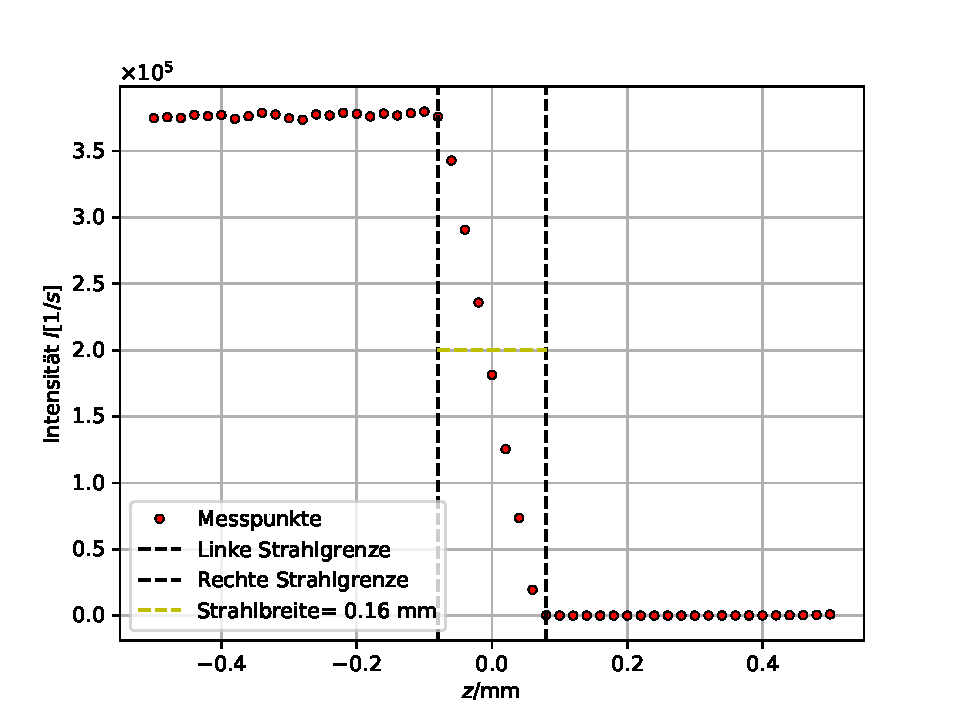
\includegraphics[width=0.8\textwidth]{plots/Zscan.pdf}
    \caption{Z-Scan zur Bestimmung der Strahlbreite}
    \label{fig:Zscan}
\end{figure}

\begin{figure}[H]
    \centering
    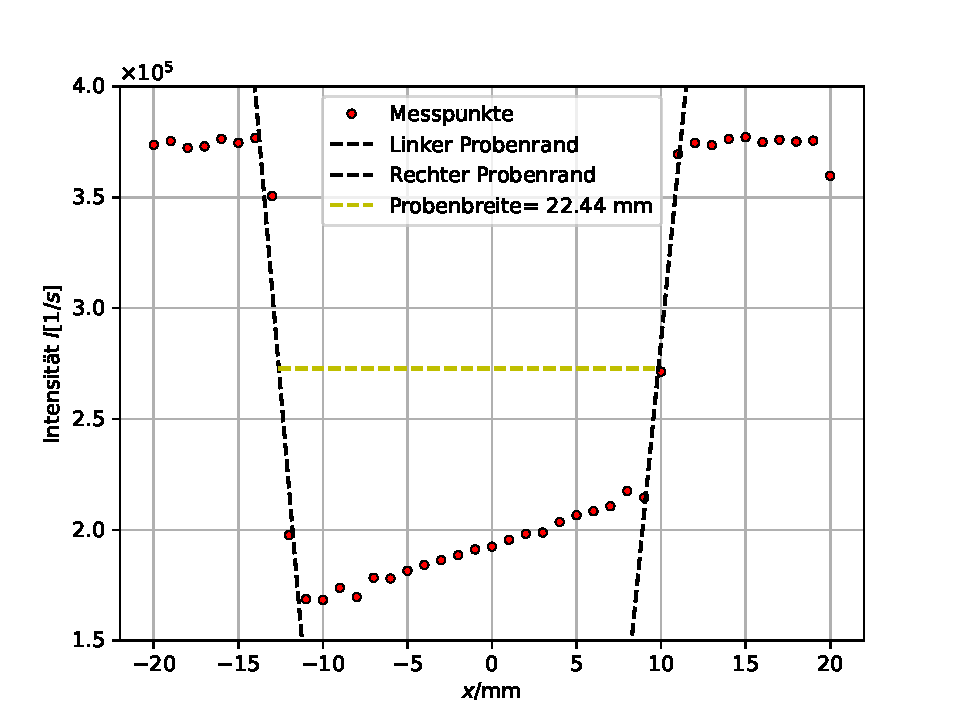
\includegraphics[width=0.8\textwidth]{plots/Xscan.pdf}
    \caption{X-Scan zur Bestimmung der Probenbreite}
    \label{fig:Xscan}
\end{figure}

\begin{figure}[H]
    \centering
    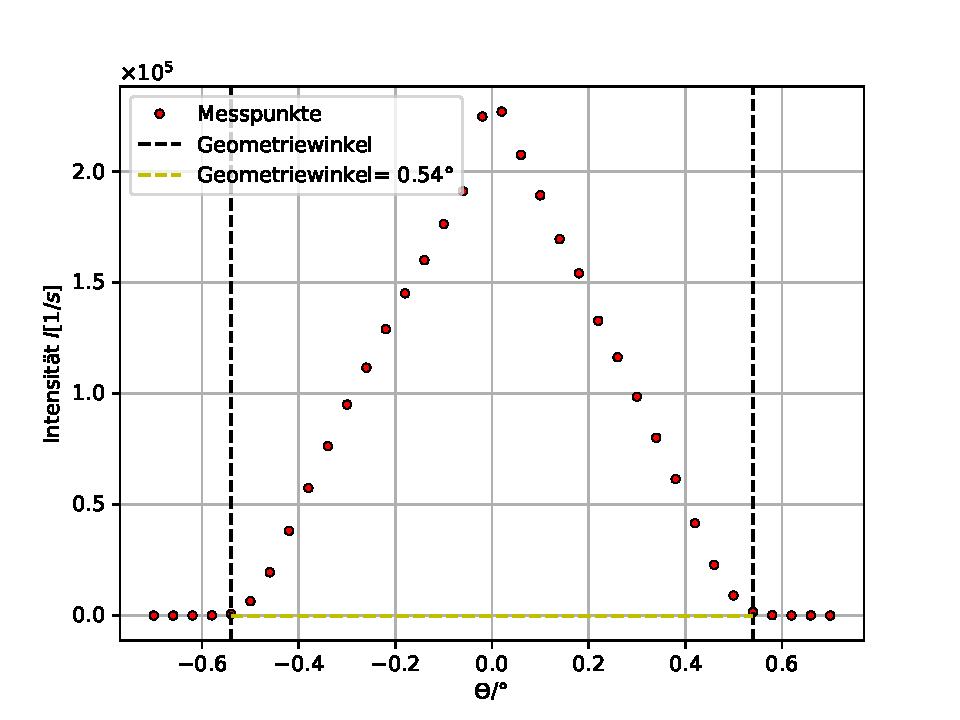
\includegraphics[width=0.8\textwidth]{plots/Rocking.pdf}
    \caption{Rockingscan zur Bestimmung des Geometriewinkels}
    \label{fig:Rocking}
\end{figure}
\subsection{Bestimmung der Rauigkeit und des Brechungsindex von Grenzschichten}
\begin{figure}[H]
    \centering
    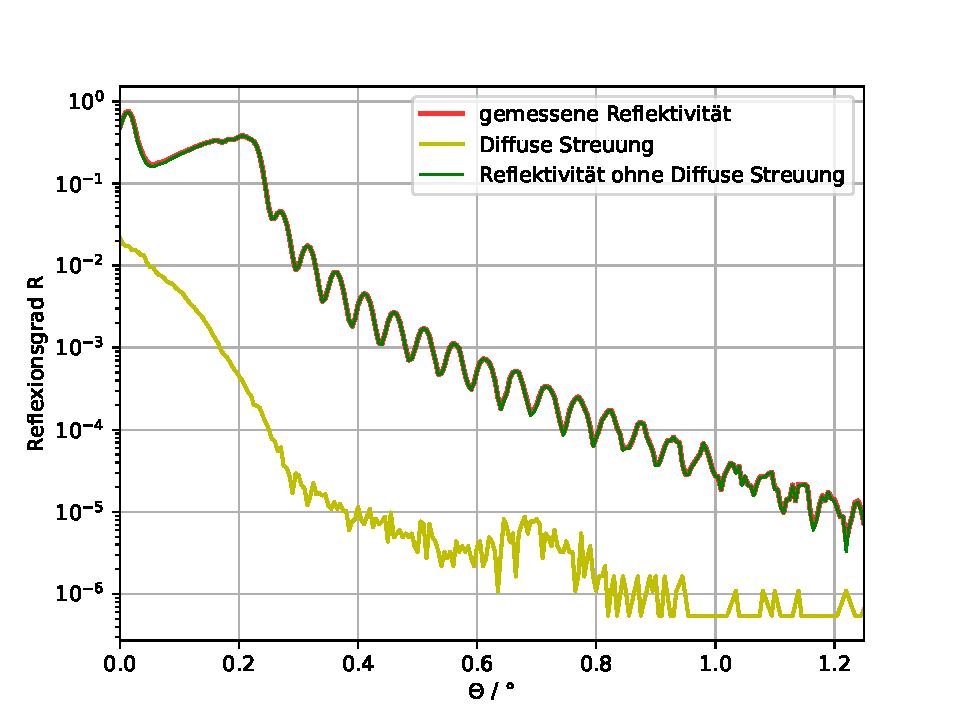
\includegraphics[width=0.8\textwidth]{plots/Reflektionsmessung.pdf}
    \caption{Reflexionsmessung in Abhängigkeit des Einfallswinkels}
    \label{fig:Reflektionsmessung}
\end{figure}

\begin{figure}[H]
    \centering
    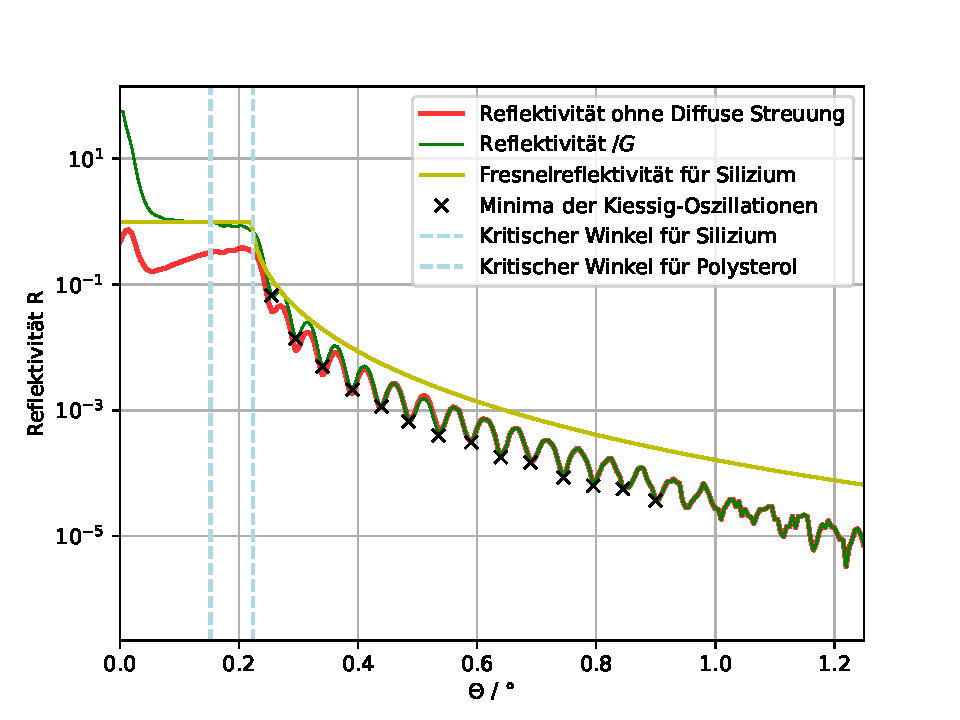
\includegraphics[width=0.8\textwidth]{plots/KorrigierteReflektionsmessung.pdf}
    \caption{Geometriefaktorkorrektur der Reflexionsmessung}
    \label{fig:KorrigierteReflektionsmessung}
\end{figure}

\begin{figure}[H]
    \centering
    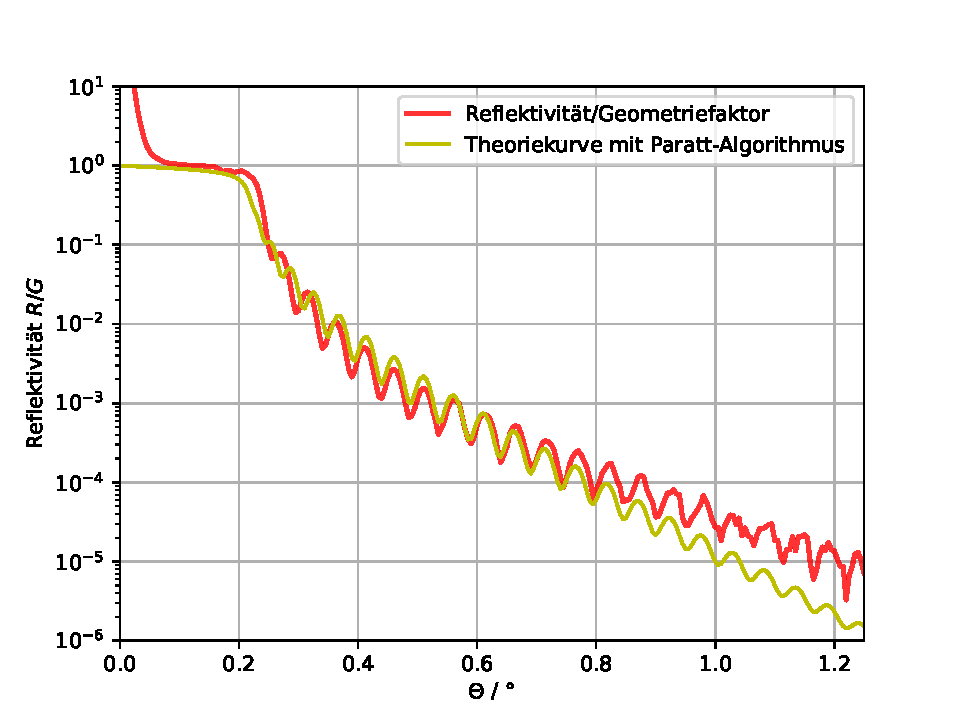
\includegraphics[width=0.8\textwidth]{plots/Parattplot.pdf}
    \caption{Näherung der Fresnelreflektivität durch das Paratt-Modell}
    \label{fig:Parattplot}
\end{figure}



